% !TEX root = rob1.tex
\chapter{Autonome Roboter}

\section{Überblick}
\subsection{Fähigkeiten eines autonomen Robotersystems}
\begin{figure}[!h]
    \centering
    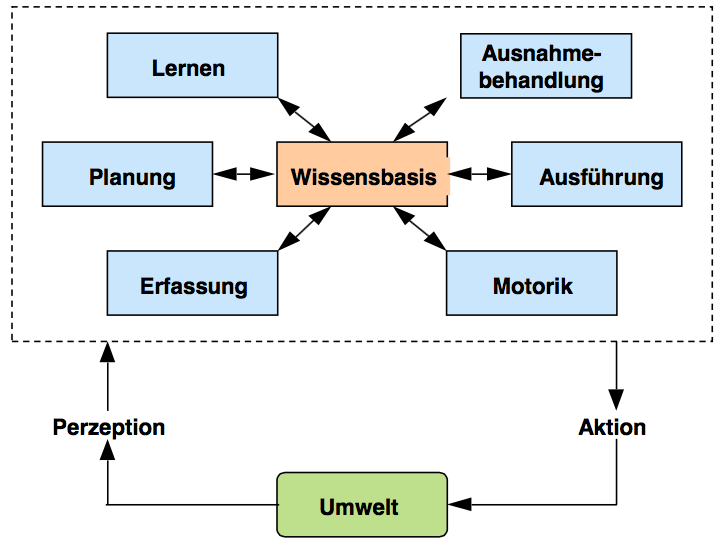
\includegraphics [scale=0.3]{faehig}
\end{figure}

\subsection{Architekturübersicht}
\begin{figure}[!h]
    \centering
    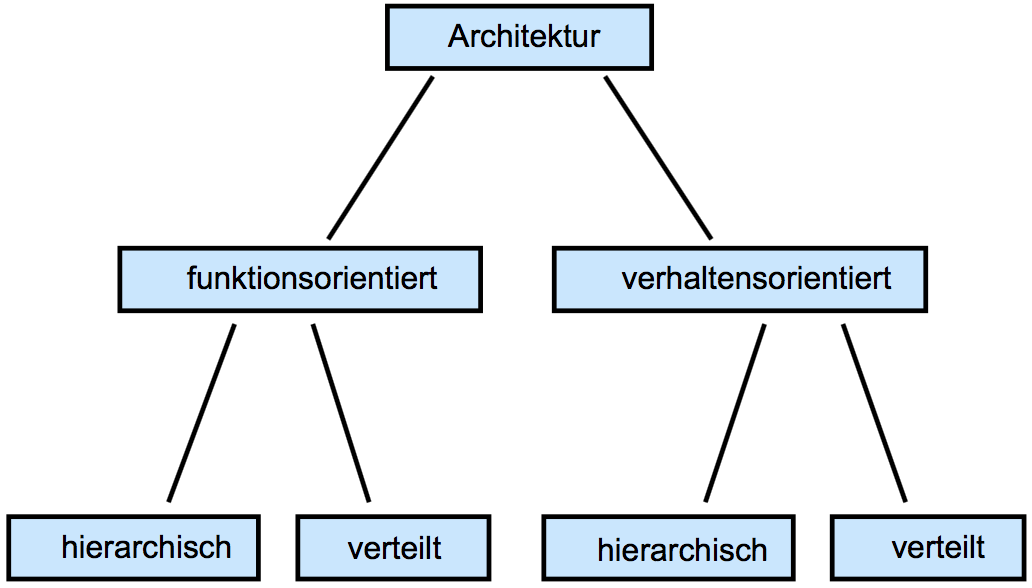
\includegraphics [scale=0.3]{architektur}
\end{figure}

\section{Funktionsorientierte Architektur}
\subsection{Genereller Aufbau}
\begin{figure}[!h]
    \centering
    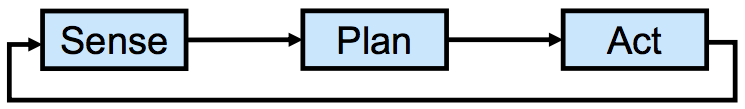
\includegraphics [scale=0.8]{generel}
    \caption{Sense Plan Act Architektur}
\end{figure}

\begin{compactitem}
    \item Unidirektionaler Informationsfluss
    \item Schlecht für dynamisch Umgebung, Interaktion
    \item Einfacher Aufbau
\end{compactitem}

\subsection{Hierarchische funktionsorientierte Architekturen}
\mparagraph{NASREM}
\begin{compactitem}
    \item Aufteilung in 4 bis 6 Ebenen
    \item pro Ebene 3 sog. Module
    \begin{compactitem}
        \item $G_i$ Sensorverarbeitungsmodul
        \item $M_i$ Weltmodell und Referenzdatenmodul
        \item $H_i$ Taskzerlegungs, Planungsund Ausfführungsmodul
    \end{compactitem}
    \item Jede Modulart ist durch dei Ebeneneinteilung hierarchisch geordnet
\end{compactitem}
\begin{figure}[!h]
    \centering
    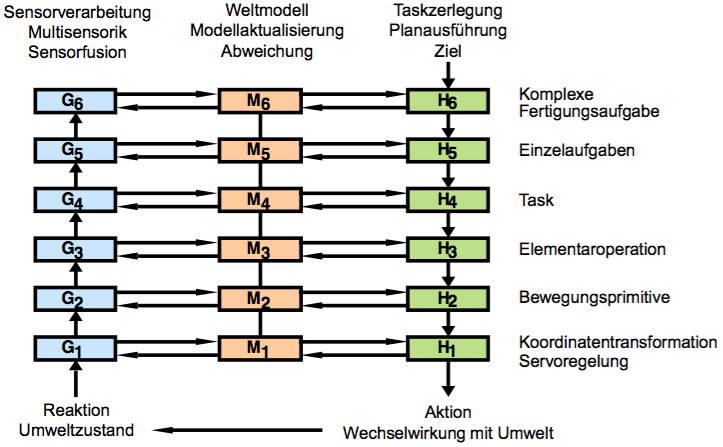
\includegraphics [scale=0.4]{nasrem}
\end{figure}
\begin{figure}[!h]
    \centering
    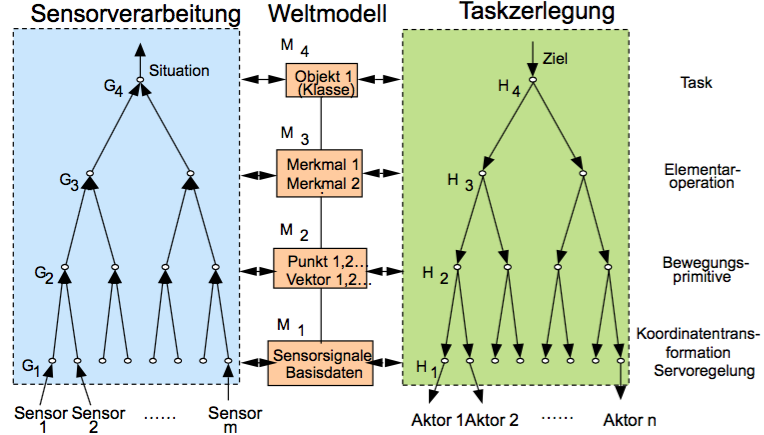
\includegraphics [scale=0.4]{nasreminfo}
\end{figure}

\mparagraph{H Modul}
\begin{compactitem}
    \item Erhält Aufgaben aus der oberen Ebene
    \item Mit Daten aus M Modul wird Aufgabe in Teilaufgaben zerlegt
    \item M Modul wird aktualisiert
    \item Teilaufgaben werden einzeln an die untere Ebene weitergereicht
\end{compactitem}
\mparagraph{G Modul}
\begin{compactitem}
    \item Bekommt Sensor Information aus der unteren Ebene
    \item Daten werden mit M Modul verarbeitet
    \item M Modul wird aktualisiert
    \item Informationen werden der oberen Ebene zur Verfügung gestellt
\end{compactitem}
\mparagraph{M Modul}
\begin{compactitem}
    \item Besteht aus einer einzigen Komponenten, mit der G und H Module Daten
    mit dem Abstraktionsgrad der jeweiligen Ebene austauschen
    \item Störung wird durch eine Differenz der Solldaten (M Modul) und den
    IstDaten (G Modul) erkannt.
\end{compactitem}
\subsection{Verteilt funktionsorientierte Architekturen}
\begin{compactitem}
    \item Menge spezialisierter Teilsysteme
    \item Kommunikation über eine zentrale Komponente
\end{compactitem}
\section{Verhaltensorientierte Architektur}
\subsection{Hierarchische funktionsorientierte Architekturen}
\begin{compactitem}
    \item hierarchische Anordnung in Verhaltensebenen der Einzelverhalten
    \item Übergeordnete Verhalten können die Ausgabe darunter liegender Verhalten
    hemmen
    \item Steuerung durch Verhaltensmuster bzw. Reflexe
    \item Muster: reaktion des Systems auf bestimmte Sensorstimuli (Umweltsituation)
\end{compactitem}
\subsection{Verteilt funktionsorientierte Architekturen}
\begin{compactitem}
    \item Menge von unabhängigen Teilsystemen mit identischen Verhaltensmustern
    \item Koordination erfolgt über ein Verhaltensmuster
\end{compactitem}
